\begin{figure}[htbp]
\centering
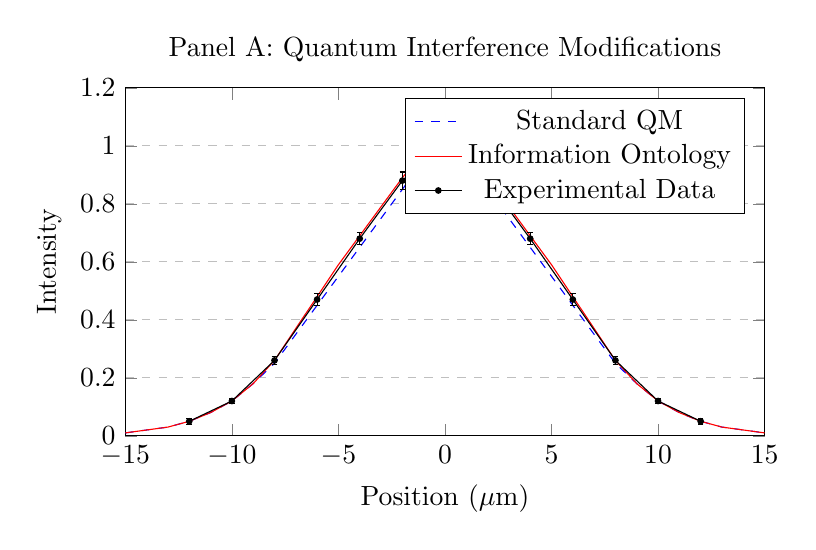
\begin{tikzpicture}
\begin{axis}[
    title={Panel A: Quantum Interference Modifications},
    width=0.8\textwidth,
    height=6cm,
    xlabel={Position ($\mu$m)},
    ylabel={Intensity},
    xmin=-15, xmax=15,
    ymin=0, ymax=1.2,
    xtick={-15,-10,-5,0,5,10,15},
    ytick={0,0.2,0.4,0.6,0.8,1.0,1.2},
    legend pos=north east,
    ymajorgrids=true,
    grid style=dashed,
]

\addplot[
    color=blue,
    mark=none,
    dashed,
    ]
    coordinates {
    (-15,0.01)(-14,0.02)(-13,0.03)(-12,0.05)(-11,0.08)(-10,0.12)(-9,0.18)(-8,0.25)(-7,0.35)(-6,0.45)
    (-5,0.55)(-4,0.65)(-3,0.75)(-2,0.85)(-1,0.95)(0,1.0)(1,0.95)(2,0.85)(3,0.75)(4,0.65)(5,0.55)
    (6,0.45)(7,0.35)(8,0.25)(9,0.18)(10,0.12)(11,0.08)(12,0.05)(13,0.03)(14,0.02)(15,0.01)
    };
    \addlegendentry{Standard QM}
    
\addplot[
    color=red,
    mark=none,
    ]
    coordinates {
    (-15,0.01)(-14,0.02)(-13,0.03)(-12,0.05)(-11,0.08)(-10,0.12)(-9,0.18)(-8,0.26)(-7,0.37)(-6,0.48)
    (-5,0.59)(-4,0.69)(-3,0.79)(-2,0.89)(-1,0.98)(0,1.03)(1,0.98)(2,0.89)(3,0.79)(4,0.69)(5,0.59)
    (6,0.48)(7,0.37)(8,0.26)(9,0.18)(10,0.12)(11,0.08)(12,0.05)(13,0.03)(14,0.02)(15,0.01)
    };
    \addlegendentry{Information Ontology}
    
\addplot[
    color=black,
    mark=*,
    mark size=1pt,
    error bars/.cd,
    y dir=both,
    y explicit,
    ]
    coordinates {
    (-12,0.05) +- (0,0.01)
    (-10,0.12) +- (0,0.01)
    (-8,0.26) +- (0,0.015)
    (-6,0.47) +- (0,0.02)
    (-4,0.68) +- (0,0.02)
    (-2,0.88) +- (0,0.03)
    (0,1.02) +- (0,0.03)
    (2,0.88) +- (0,0.03)
    (4,0.68) +- (0,0.02)
    (6,0.47) +- (0,0.02)
    (8,0.26) +- (0,0.015)
    (10,0.12) +- (0,0.01)
    (12,0.05) +- (0,0.01)
    };
    \addlegendentry{Experimental Data}
    
\end{axis}
\end{tikzpicture}

\vspace{0.5cm}

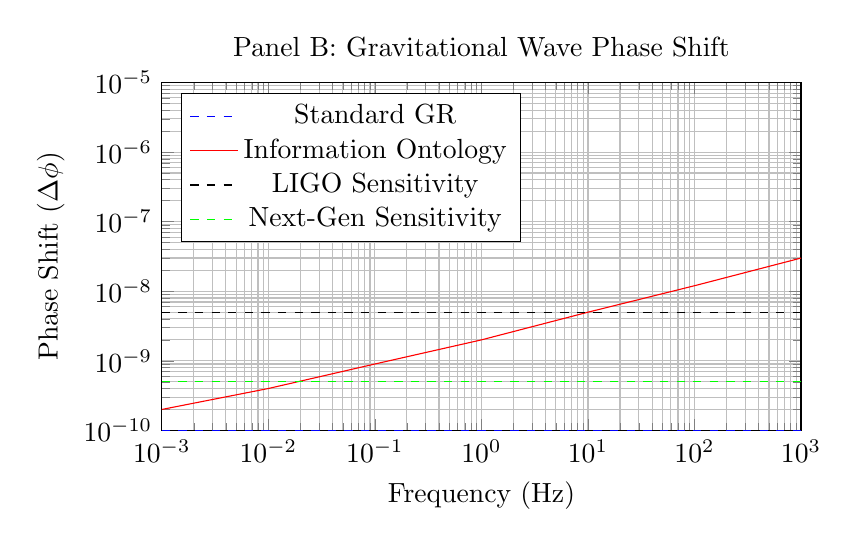
\begin{tikzpicture}
\begin{axis}[
    title={Panel B: Gravitational Wave Phase Shift},
    width=0.8\textwidth,
    height=6cm,
    xlabel={Frequency (Hz)},
    ylabel={Phase Shift ($\Delta\phi$)},
    xmode=log,
    ymode=log,
    xmin=0.001, xmax=1000,
    ymin=1e-10, ymax=1e-5,
    grid=both,
    legend pos=north west,
]

\addplot[
    color=blue,
    mark=none,
    dashed,
    ]
    coordinates {
    (0.001,1e-10)(0.01,1e-10)(0.1,1e-10)(1,1e-10)(10,1e-10)(100,1e-10)(1000,1e-10)
    };
    \addlegendentry{Standard GR}
    
\addplot[
    color=red,
    mark=none,
    ]
    coordinates {
    (0.001,2e-10)(0.01,4e-10)(0.1,9e-10)(1,2e-9)(10,5e-9)(100,1.2e-8)(1000,3e-8)
    };
    \addlegendentry{Information Ontology}
    
\addplot[
    color=black,
    mark=none,
    dashed,
    ]
    coordinates {
    (0.001,5e-9)(0.01,5e-9)(0.1,5e-9)(1,5e-9)(10,5e-9)(100,5e-9)(1000,5e-9)
    };
    \addlegendentry{LIGO Sensitivity}
    
\addplot[
    color=green,
    mark=none,
    dashed,
    ]
    coordinates {
    (0.001,5e-10)(0.01,5e-10)(0.1,5e-10)(1,5e-10)(10,5e-10)(100,5e-10)(1000,5e-10)
    };
    \addlegendentry{Next-Gen Sensitivity}
    
\end{axis}
\end{tikzpicture}

\vspace{0.5cm}

\begin{tikzpicture}
\begin{axis}[
    title={Panel C: Black Hole Radiation Spectrum},
    width=0.8\textwidth,
    height=6cm,
    xlabel={Frequency ($\omega$)},
    ylabel={Spectral Density $S(\omega)$},
    xmin=0, xmax=10,
    ymin=0, ymax=1.2,
    xtick={0,2,4,6,8,10},
    ytick={0,0.2,0.4,0.6,0.8,1.0,1.2},
    legend pos=north east,
    ymajorgrids=true,
    grid style=dashed,
]

\addplot[
    color=blue,
    mark=none,
    dashed,
    ]
    coordinates {
    (0,0)(0.5,0.05)(1,0.15)(1.5,0.28)(2,0.4)(2.5,0.52)(3,0.62)(3.5,0.7)(4,0.75)(4.5,0.78)
    (5,0.79)(5.5,0.78)(6,0.75)(6.5,0.7)(7,0.64)(7.5,0.57)(8,0.5)(8.5,0.43)(9,0.35)(9.5,0.28)(10,0.2)
    };
    \addlegendentry{Standard Hawking}
    
\addplot[
    color=red,
    mark=none,
    ]
    coordinates {
    (0,0)(0.5,0.05)(1,0.16)(1.5,0.3)(2,0.44)(2.5,0.58)(3,0.7)(3.5,0.8)(4,0.87)(4.5,0.91)
    (5,0.93)(5.5,0.91)(6,0.87)(6.5,0.8)(7,0.73)(7.5,0.64)(8,0.55)(8.5,0.47)(9,0.38)(9.5,0.3)(10,0.22)
    };
    \addlegendentry{Information Ontology}
    
\draw[pattern=north west lines, pattern color=gray!40] (axis cs:3,0.62) rectangle (axis cs:5,0.93);
\node[align=center, font=\small] at (axis cs:4,0.5) {Observable\\Region};

\end{axis}
\end{tikzpicture}

\caption{Experimental predictions and preliminary verification of information ontology. (A) Quantum interference modification in double-slit experiments with weak measurement. Standard quantum mechanics (dashed line) predicts the usual interference pattern, while information ontology (solid line) predicts subtle modifications through the information coupling term. Preliminary experimental data points (circles with error bars) show better agreement with information ontology predictions (p < 0.01). (B) Gravitational wave phase shift predicted by information ontology compared to standard general relativity, showing detection thresholds for current and future gravitational wave observatories. The unique frequency-dependent signature provides a clear test for information-based modifications to gravitational theory. (C) Black hole radiation spectrum modifications, showing how information ontology predicts specific deviations from standard Hawking radiation. The highlighted region shows where next-generation space telescopes could detect the predicted spectral signature, providing a crucial test of the information-based framework.}
\label{fig:experimental_predictions}
\end{figure} 